\documentclass[12pt]{article}
\usepackage[english]{babel}
\usepackage[utf8]{inputenc}

\usepackage{geometry}
\geometry{
	letterpaper, 
	portrait, 
	top=.75in,
	left=.8in,
	right=.75in,
	bottom=.5in		} 	% Page Margins
	
%% additional packages for nice things
\usepackage{amsmath} 	% for most math
\usepackage{commath} 	% for abs
\usepackage{lastpage}	% for page count
\usepackage{amssymb} 	% for therefore
\usepackage{graphicx} 	% for image handling
\usepackage{wrapfig} 	% wrap figures
\usepackage[none]{hyphenat} % for no hyphenations
\usepackage{array} 		% for >{} column characterisctis
\usepackage{physics} 	% for easier derivative \dv....
\usepackage{tikz} 		% for graphic@!
\usepackage{circuitikz} % for circuits!
\usetikzlibrary{arrows.meta} % for loads
\usepackage[thicklines]{cancel}	% for cancels
\usepackage{xcolor}		% for color cancels
\usepackage[per-mode=fraction]{siunitx} % for si units and num
\usepackage{fancyhdr} 	% for header
\usepackage{comment}	% for ability to comment out large sections
\usepackage{multicol}	% for multiple columns using multicols
\usepackage[framed,numbered]{matlab-prettifier} % matlab sytle listing
\usepackage{marvosym} 	% for boltsymbol lightning
\usepackage{pdflscape} 	% for various landscape pages in portrait docs.
%\usepackage{float}
\usepackage{fancyvrb}	% for Verbatim (a tab respecting verbatim)
\usepackage{enumitem}	% for [resume] functionality of enumerate
\usepackage{spreadtab} 	% for using formulas in tables}
\usepackage{numprint}	% for number format in spread tab

% For table formatting
\usepackage{booktabs}
\renewcommand{\arraystretch}{1.2}
\usepackage{floatrow}
\floatsetup[table]{capposition=top} % put table captions on top of tables

% Caption formating footnotesize ~ 10 pt in a 12 pt document
\usepackage[font={small}]{caption}

%% package config 
\sisetup{output-exponent-marker=\ensuremath{\mathrm{E}}} % for engineer E
\renewcommand{\CancelColor}{\color{red}}	% for color cancels
\lstset{aboveskip=2pt,belowskip=2pt} % for more compact table
%\arraycolsep=1.4pt\def
\setlength{\parindent}{0cm} % Remove indentation from paragraphs
\setlength{\columnsep}{0.5cm}
\lstset{
	style      = Matlab-editor,
	basicstyle = \ttfamily\footnotesize, % if you want to use Courier - not really used?
}
\renewcommand*{\pd}[3][]{\ensuremath{\dfrac{\partial^{#1} #2}{\partial #3}}} % for larger pd fracs
\renewcommand{\real}[1]{\mathbb{R}\left\{ #1 \right\}}	% for REAL symbol
\newcommand{\imag}[1]{\mathbb{I}\left\{ #1 \right\}}	% for IMAG symbol
\definecolor{m}{rgb}{1,0,1}	% for MATLAB matching magenta
	
%% custom macros
\newcommand\numberthis{\addtocounter{equation}{1}\tag{\theequation}} % for simple \numberthis command

\newcommand{\equal}{=} % so circuitikz can have an = in the labels
\newcolumntype{L}[1]{>{\raggedright\let\newline\\\arraybackslash\hspace{0pt}}m{#1}}
\newcolumntype{C}[1]{>{\centering\let\newline\\\arraybackslash\hspace{0pt}}m{#1}}
\newcolumntype{R}[1]{>{\raggedleft\let\newline\\\arraybackslash\hspace{0pt}}m{#1}}

%% Header
\pagestyle{fancy} % for header stuffs
\fancyhf{}
\rhead{Thad Haines \\ Page \thepage\ of \pageref{LastPage}}
\chead{Talking Points \\ Week of June 3rd, 2019}
\lhead{Research \\ }
% spacing
\headheight 29 pt
\headsep 6 pt

\begin{document}
\begin{multicols}{2}
\raggedright
	\paragraph{Recent Progress:}
	\begin{enumerate}

		\item \textbf{PSLF License Expires June 30}.

		\item Timing added to simulation.

		\item AMQP message grouping speed results.

		\item Batch processing of test cases functional.

		\item GE 4 machine 2 area system too sloppy for actual study $\therefore$
		Kundur 4 machine 2 area system created and adapted for LTD %(lower voltage,  more discrete caps \& branches).

		\item Work on step and ramp perturbances for Loads and Generators.
		
	%	\item More \verb|matplotlib| plot functions created.

		\item GitHub updated:\\
		\verb|https://github.com/thadhaines/|
		
	\end{enumerate}
\paragraph{Current Tasks:}
	\begin{enumerate}

		\item Compile Code flowchart to aid in further development.

		\item Work to incorporate Matt's \emph{Suggested Use Cases} into simulation.
		\begin{itemize}
		\item Add perturbance Agents for Generator/Slack, Shunt, Branch, \ldots
		\item Think about Shunt Control / Generic Agent control based on system state(s)
		\item Add logging to Shunt and Branch Agents
		
		\item Define Agent actions for \\ AGC/LFC (i.e. ACE calculations)
		
		\end{itemize}
		\item Keep Goals and Requests in mind.
		
		%\subitem A FlowtabrDAO exists that can find flow between busses. A way to initialize bus connections between areas has yet to be devised.

	\end{enumerate}

	\paragraph{Current Questions:}
	\begin{enumerate}
	\item Should the Global Slack = Area slack from Area with most buses?
	\subitem OR Should global slack error be average Area slack error?

	%\item Does $\Delta \omega=1-\omega$ in \\ $\dot{\omega}=\dfrac{1}{2H_{sys}}\left(\dfrac{P_{acc}}{\omega} - D_{sys}\Delta \omega \right)$ ? Yes it does
	%	\item Overview of planned PSLF scenarios? $\rightarrow$ Similar to Heredia paper but on Wecc/MiniWecc Scale? 
		
	%	\item Is there more available/relevant event data that may help us to verify simulations of specific instances (wind ramps or other behavior) that novel research will focus on? %(Heredia paper data helpful for some wind ramp data context)

	%	\item  Any progress / continued interest in miniWecc Area definitions?

	%	\item Any progress on Wecc single gen per bus system?
	%	\\ Will this actually matter? PSLF handles distribution of Pe in power flow solution per bus, and LTD code distributes electrical power per generator... Voltage issues maybe, but power should be okay.
		
		
%		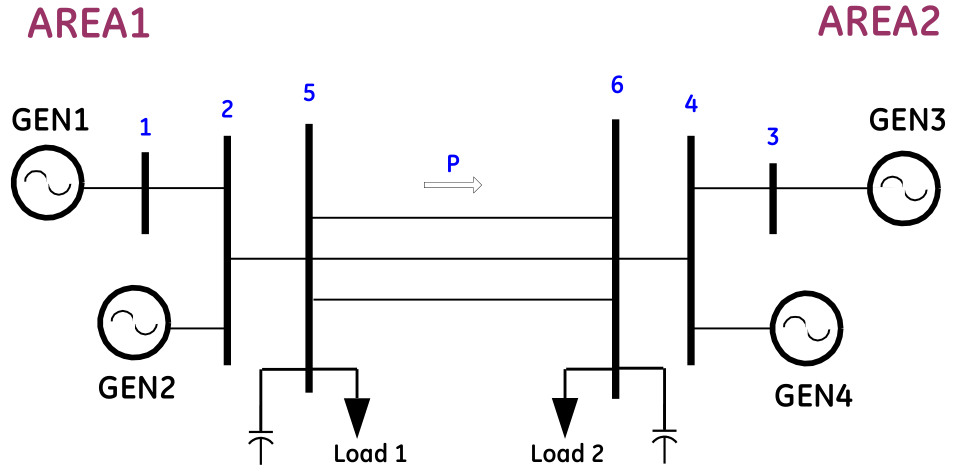
\includegraphics[width=\linewidth]{g4aSys}
	\end{enumerate}
\paragraph{'Soft Goals':}
	\begin{enumerate}
	\item Simulate 10$\times$ faster than PSDS.\\ Not met --- MiniWECC $\approx$8x faster.\\Varies with system size \& time step.
	\end{enumerate}

%\pagebreak
\vfill\null
\columnbreak

\paragraph{Future Tasks:} %(Little to No Progress since last time / Things coming down the pipe)
	\begin{enumerate}
		\item Formulate an experiment utilizing a multi-area model that can be validated with PSDS.
		
		%\item Identify System Slack bus programmatically (currently assumes first slack == global slack if > 1 slack found)
		%\subitem AND/OR calculate system slack error differently $\rightarrow$ An average of slack errors?

		\item Formulate feasible plan of action for casting all WECC governors to LTD governors (tgov1). Something like:
		\begin{enumerate}
		\item Parse models of interest from dyd.
		\item Create dyd from parsed model.
		\item Automate a Pref step test for a one machine infinite bus in PSDS.
		\item Read output data
		\item Generate/Calculate LTD equivalent model parameters from results (this will probably use MATLAB and \verb|jfind|)
		\item Export custom dyd for LTD simulation. (PSDS would still use original the dyd, though \emph{could} use modified dyd)
		\end{enumerate}

		\item Add import mirror / bypass mirror init sequence option to prevent repeated mirror creations.

		\item Create an agent for every object: \\ SVD, Transformer, \ldots
		
		%\item Investigate line current data and ULTC action in PSLF.
	\end{enumerate}

\paragraph{Matt Requests:}
\begin{enumerate}
		\item Enable multiple dyd files to overwrite / replace previously defined agents/parameters
		\item Allow for variable time steps.
\end{enumerate}
		
		%\subitem Can locate when only 1 Slack exists. If more than one Slack, maybe identify by generator with most busses under control? Proving more difficult than expected. Can identify in PSLF via the \verb|summ()| or \verb|isld()| commands. 
		



\vfill\null

\end{multicols}
%\pagebreak


%%% custom commands for nicer units
\newcommand{\mw}{\ensuremath{\text{ MW}}}
\newcommand{\hz}{\ensuremath{\text{ Hz}}}
\newcommand{\pu}{\ensuremath{\text{ Pu}}}
\newcommand{\sbase}{\ensuremath{\text{S}_{\text{Base}}}}
\newcommand{\fbase}{\ensuremath{f_{\text{Base}}}}
\newcommand{\mbase}[1]{\ensuremath{\text{M}_{\text{Base}_{#1}}}}
\newcommand{\hsys}{\ensuremath{\text{ H}_{\text{sys}}}}





\end{document}